\chapter{Results}
In the previous chapter we explained the implementation details of our motion segmentation pipeline. In particular we described the purpose of every individual pipeline component and how they are implemented. \\ \\
In summary, our pipeline consists of the following main stages: generate optical flow estimations, track motion trajectories using these flow fields, compute similarities between every trajectory pair with respect to certain measures and last, perform a segmentation by clustering the trajectories according to their similarities. Every such stages offers various implementation variants, from which a user can select from. A complete list of all pipeline mode abbreviations is provided in Table $\ref{tab:pipeline_abbreviations}$. In the following \enquote{a specific stage implementation} is called \textit{pipeline mode} and \enquote{a set of pipeline modes} is called \textit{pipeline combinations}.
\begin{table}[H]
\centering
\resizebox{\columnwidth}{!}{%
\begin{tabular}{|c|c|c|}
\hline
\multicolumn{3}{|c|}{\textbf{Pipeline Abbreviations}}                                                                                                                                                                                                     \\ \hline
\textbf{Flow Methods (Sec. $\ref{sec:generate_of}$)}                                                                 & \textbf{Similarity Measures (Sec. $\ref{sec:affinity_matrix_impl}$)}                                                             & \textbf{Segmentation Techniques (Sec. $\ref{sec:sparse_motion_segmentation}$)}                                       \\ \hline
\begin{tabular}[c]{@{}c@{}}Horn and Schnunk (\textbf{HS})\\ (Page $\pageref{sec:hs_flows}$)\end{tabular}                   & \begin{tabular}[c]{@{}c@{}}Product of Distances (\textbf{PD})\\ (Eq. $\ref{eq:prod_combination}$)\end{tabular}                   & \begin{tabular}[c]{@{}c@{}}Spectral Clustering (\textbf{SC})\\ (Sec. $\ref{sec:spectral_clustering_impl}$)\end{tabular} \\ \hline
\begin{tabular}[c]{@{}c@{}}Large Displacement Optical Flows (\textbf{LDOF})\\ (Page $\pageref{sec:ldof_flows}$)\end{tabular} & \begin{tabular}[c]{@{}c@{}}Product of Distances with Depths (\textbf{PED})\\ (Eq. $\ref{eq:prod_combination}$)\end{tabular} & \begin{tabular}[c]{@{}c@{}}MinCut (\textbf{MC})\\ (Sec. $\ref{sec:min_cut_seg}$)\end{tabular}              \\ \hline
\begin{tabular}[c]{@{}c@{}}Layered RGB-D Flow Estimation (\textbf{LRGBD})\\ (Page $\pageref{sec:lrgbd_flows}$)\end{tabular}   & \begin{tabular}[c]{@{}c@{}}Sum of Distances (\textbf{SD})\\ (Eq. $\ref{eq:sum_dist}$)\end{tabular}                      & \begin{tabular}[c]{@{}c@{}}Kernighan-Lin (\textbf{KL})\\ (Sec. $\ref{sec:kl_impl}$)\end{tabular}       \\ \hline
\begin{tabular}[c]{@{}c@{}}Semi Rigid Scene Flows (\textbf{SRSF})\\ (Page $\pageref{sec:srsf_flows}$)\end{tabular}           & \begin{tabular}[c]{@{}c@{}}Sum of Distances with Depths (\textbf{SED})\\ (Eq. $\ref{eq:sum_dist}$)\end{tabular}         &                                                                        \\ \hline
\end{tabular}
}
\caption[List of Pipeline Abbreviations]{A list of all implemented pipeline modes and their abbreviations. A pipeline mode is formed by combining one flow method, together with one similarity measure and one segmentation technique.}
\label{tab:pipeline_abbreviations}
\end{table}
In this chapter we describe how we evaluate segmentations produced by different pipeline combinations. In particular, we examine the influence of several pipeline modes on the segmentation quality. \\ \\
We start be defining the default pipeline parameter specifications (Sec. $\ref{sec:spectral_clustering_parameters}$) of specific implementations. Next, we introduce the datasets (Sec. $\ref{sec:datasets}$) we use during our evaluation. In the following we describe our cluster merger post-processing step (Sec. $\ref{sec:seg_merger}$), which has to be run before starting the evaluation. We continue by describing our methodology (Sec. $\ref{sec:methodology}$) we rely on to perform the experiments. Finally, we describe our experiments (Sec. $\ref{sec:experiments}$), the corresponding results and observations. We conclude this chapter by listing some pipeline runtime measurements (Sec. $\ref{sec:runtime_measurements}$) and a discussion about our main findings (Sec. $\ref{sec:discussion}$). 

\section{Default Parameter Assignments}
\label{sec:spectral_clustering_parameters}
Even though our pipeline mainly consists of tree main components, that is the flow computation stage, the affinity matrix generation stage and the segmentation stage, it exhibits a large amount of parameters that have to be specified. This issues makes it tedious to use our implementation, especially, when having to run the pipeline repeatedly while using different modes (e.g. during our experiments). Therefore, we aim at reducing the number of free parameters in our pipeline by providing certain default assignments. \\ \\
In this section we address this problem of default parameter assignments. In particular we explain which parameter gets what default value assigned to and why. \\ \\
Our motion segmentation pipeline exhibits many parameters since it consists of several stages such as the flow generation-, affinity matrix computation-, segmentation stage. Moreover, every stage implements different techniques to approach its specified tasks. Hence, a user has to specify both, which pipeline combination should be run and what parameter values of an specific method should be used. To get the overall picture of this complexity we illustrate all available \textit{pipeline combinations} in Figure $\ref{fig:pipeline_combinations}$.
\begin{figure}[H]
\begin{center}
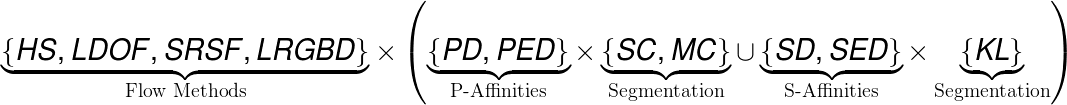
\includegraphics[width=1\linewidth] {evaluation/pipeline_combinations}
\end{center}
\caption[Pipeline Combinations]{A listing of all available pipeline combinations. Our pipeline implements a series of flow methods (4), various affinity computation modes (4) and different segmentation techniques (3). In total, there are $4 \times (2 \times 2 + 2 \times 1) = 24$ different combinations available. However, not every component mode can be combined with any other. For example \textit{S-affinities} can only be used in combination with the \textit{Kernighan-Lin Heuristic} (KL). A listing of all these combination acronyms and their meaning is given in Table $\ref{tab:pipeline_abbreviations}$.}
\label{fig:pipeline_combinations}
\end{figure}
In the following we give a brief description of several default assignments used in different pipeline stages. \\ \\
For generating the flow fields we rely on existing implementations as described in Section $\ref{sec:generate_of}$. We do not attempt to modify any parameter settings while utilizing those flow methods and thus strictly rely on their default settings. A summary about these flow methods can be found in Section $\ref{sec:impl_optical_flow}$ on page $\pageref{sec:impl_optical_flow}$. \\ \\
Before tracking trajectories as described in Section $\ref{sec:trajectory_tracking}$, we initially have to extract their feature locations (Sec. $\ref{sec:tracking_candidates}$). The resulting feature extraction is determined by a parameter defining the sparsity of the sampling rate, indicating to use only every $k-th$ feature. Throughout performing our experiments we will be using $k$ equals to 8. This choice is justified by the fact that using a smaller sampling rate would not enhance the result's quality and negatively influence the overall runtime, whereas larger values would cause the opposite. \\ \\
Next some words about choosing defaults for the affinity matrix generation stage. Before computing a $\textit{P-affinity}$, either by running the mode \textit{PD} or $\textit{PED}$, we have to specify a certain value $\lambda$. This parameter is used in Equation $\ref{eq:prod_dist_affinity}$ and acts as a scale of the similarity between two trajectories. In the following we use$\footnote{We determined the defaults by trying out different values for $\lambda$ and took those which yielded the visually most promising results. Please note that this kind of parameter selection is by no means optimal.}$ $\lambda$ equals $0.01$ when running $PD$ and $\lambda = 50$ when running the affinity mode $PED$. The reason for using different $\lambda$ values is because PED and PD have different scales. As we can see $\lambda$ takes different powers to ten. However the exact choice of this scale does not matter$\footnote{Meaning, that it \textit{does not matter} regarding using a different mantissa, since it will not affect the final outcome of the affinity matrix drastically.}$ that much as long as it close to the same power to ten value as its corresponding default. \\ \\
When having a closer look at the computed affinities, we observe, that approximately one third of the trajectory neighbors have similarity large enough to have a big influence on it. Therefore, we decided to set the number of closest neighbors per trajectory equals one third of the total neighbors. An example of such affinities is shown in Figure $\ref{fig:cars_affinities}$. A dark pixel indicates a low affinity between two trajectories and bright regions indicate large affinities. \\ \\
In order to generate S-affinities we rely on the definition of Equation $\ref{eq:sum_dist}$, which is used to compute distances between trajectories. However, this equation is parameterized by several weights $\beta$. In this work we use exactly the same $\beta$ parameter values as specified in the paper $\cite{KB15b}$, which are equal to
\begin{equation}
\begin{aligned}
\bar{\beta}_0 = 6 \text{, } \beta_0 = 2 \text{, } \beta_1 = \beta_3 = -0.02 \text{ and } \beta_2 = -4
\end{aligned}
\end{equation}
In our experiments we set the dummy vertex count in the Kernighan-Lin partitioning method always equals zero. \\ \\
For every segmentation methods, we set the \textit{cluster count} \enquote{they are supposed to solve for} to two times the number of an estimated number of moving objects present in the target dataset. In other words the cluster count (\textbf{CC}) is defined as
\begin{equation}
	\text{CC} = 2 \times \text{Estimated Moving Objects in Dataset}
\label{eq:cc_def} 
\end{equation}
This estimation approach only takes into account very clearly, distinct moving objects and is thus probably underestimating the real moving object count. \\ \\
Segmentation methods that rely on P-affinities are utilizing a certain number of eigenvectors resulting from the eigenvalue decomposition of the Laplacian. For this eigenvector Count (EV) we use twice the number of the clusters the methods are supposed to solve for, i.e. this count is defined as
\begin{equation}
	\text{EV} = 2 \times \text{CC}
\end{equation}
Moreover, when using the MC segmentation, we set the default of its data- and smoothness relaxation parameter $\nu$ used by its energy term (defined in Equation $\ref{eq:min_cut_energy_revisited}$) equals to the dimension of the affinity matrix times $10^{-6}$. Again, this value has been determined by simply trying out various assignments. Furthermore, we observed that it is sufficient to run about 10-20 iterations until MC converges. Therefore, we conservatively assign the number of iterations $\text{MC}_i$ equals 20. \\ \\
Unless stated otherwise we rely on those parameter default parameter specifications to generate out results. Moreover, in Section $\ref{sec:parameter_experiments}$, we offer a statistical justification for the default choices of $\lambda$, $\text{CC}$, $\text{EV}$ and $\text{MC}_i$.

\section{Datasets}
\label{sec:datasets}
In this section we introduce the dataset we were using for generating our results. Our dataset are a diverse collection of videos, originating from various source. Some videos were captures by Microsoft's Kinect, some by Asus' Xtion. Some were manually captures and again others are from other authors. In particular the cars dataset is from the BMS-26 dataset$\footnote{See \url{http://lmb.informatik.uni-freiburg.de/resources/datasets/}}$ and datasets prefixed by \textit{Bonn} are from Bonn's RGB-D Rigid Multi-Body Dataset $\footnote{See \url{http://www.ais.uni-bonn.de/download/rigidmultibody/}}$. \\ \\
We aim to work with a diverse collection of datasets. Meaning that we want to use datasets that capture different types of motions, show indoor- and outdoor scenes and are captured by a static or moving cameras. Also, our implementation should be able to generated segmentations for long as well as for short sequences. \\ \\
Regularly, a dataset consists of the frames of a RGB-D video and the corresponding depth-and color camera calibrations. Moreover, for a selected set of frames we manually have drawn$\footnote{To draw these ground truth images using Gimp.}$ ground truth (\textbf{GT}) images. Please notice that all GT images were drawn according to the painter's opinion and thus do probably not truly correspond to the real ground truth motion. Each color in such a GT image belongs to a moving object. However, the color \textit{black} has a spacial meaning and marks pixels that are not certain to which moving object they belong to. Such pixel locations are ignored during our evaluation. \\ \\
In the following a listing of our datasets, showing three of its frames, one of its ground truth motion segmentation images, a list of properties, such as the number of estimated objects and lastly, a brief description what is happening in the video sequence:
\begin{itemize}
\item \textbf{Cars}: \\ 
\textbf{Frames}: 19, \textbf{Resolution}: $480 \times 640$, \textbf{Depths}: No, \textbf{Estimated Objects}: 3
\begin{figure}[H]
\begin{center}
\subfigure[Frame 1]{
   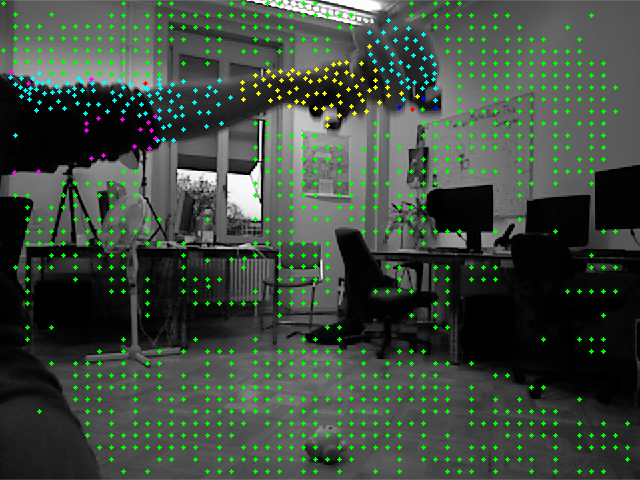
\includegraphics[width=0.22\linewidth] {evaluation/datasets/cars/1}
}
\subfigure[Frame 10]{
   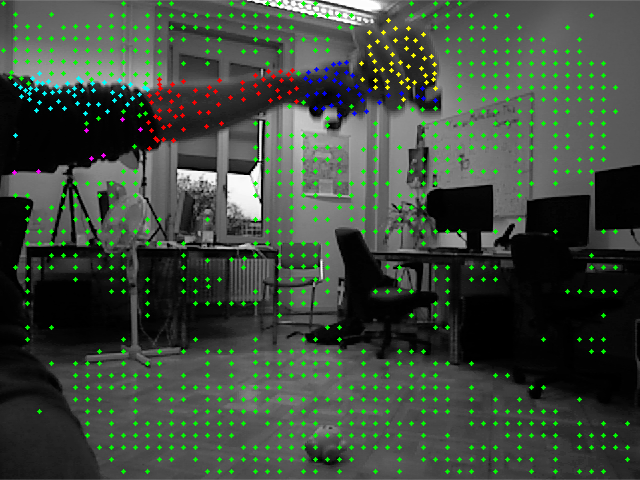
\includegraphics[width=0.22\linewidth] {evaluation/datasets/cars/10}
}
\subfigure[Frame 19]{
   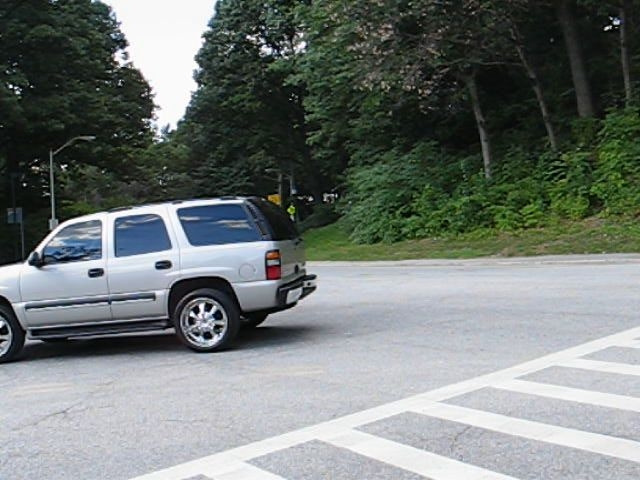
\includegraphics[width=0.22\linewidth] {evaluation/datasets/cars/19}
}
\subfigure[GT Frame 1]{
   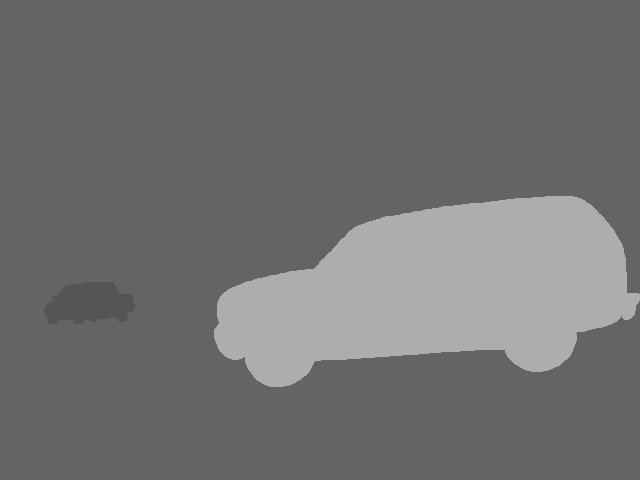
\includegraphics[width=0.22\linewidth] {evaluation/datasets/cars/gt1}
}
\end{center}
\caption[Dataset Bonn Cars]{An outdoor scene showing two cars, both moving to the left. One in the front and the other in the background. The camera is static.}
\label{fig:eval_datasets_cars}
\end{figure}
\item \textbf{Bonn Watercan}: \\
\textbf{Frames}: 58, \textbf{Resolution}: $480 \times 640$, \textbf{Depths}: Yes, \textbf{Estimated Objects}: 5
\begin{figure}[H]
\begin{center}
\subfigure[Frame 4]{
   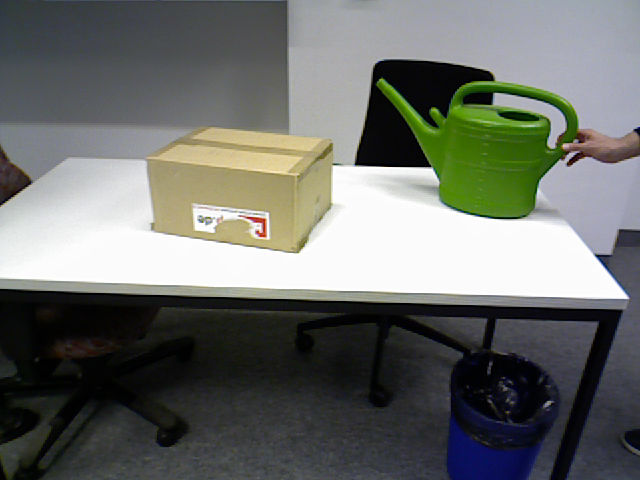
\includegraphics[width=0.22\linewidth] {evaluation/datasets/bonn_watercan/4}
}
\subfigure[Frame 31]{
   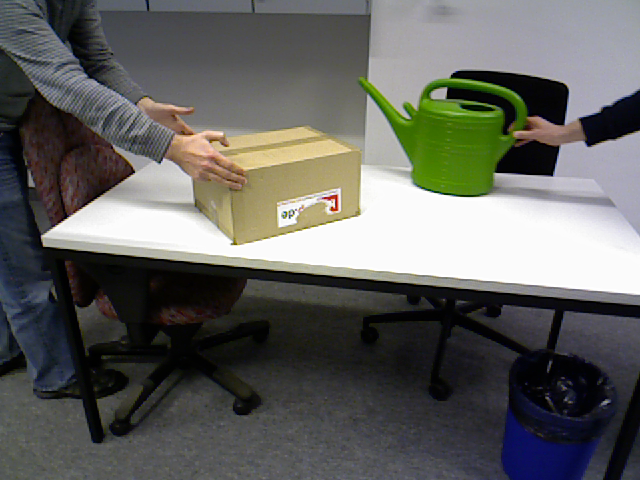
\includegraphics[width=0.22\linewidth] {evaluation/datasets/bonn_watercan/31}
}
\subfigure[Frame 58]{
   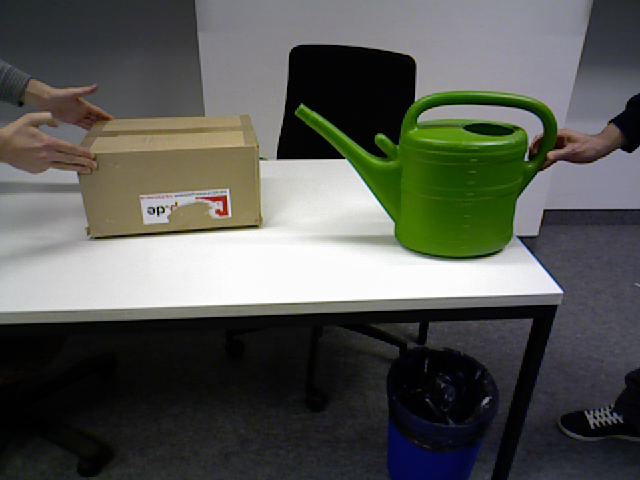
\includegraphics[width=0.22\linewidth] {evaluation/datasets/bonn_watercan/58}
}
\subfigure[GT Frame 4]{
   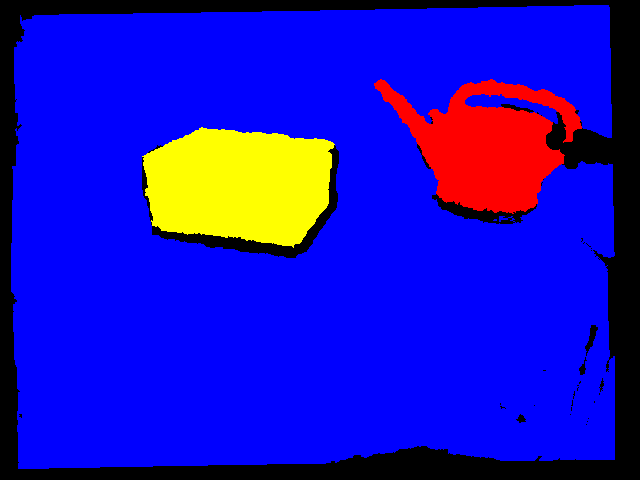
\includegraphics[width=0.22\linewidth] {evaluation/datasets/bonn_watercan/gt4}
}
\end{center}
\caption[Dataset Bonn Watercan]{An indoor scene showing two men pushing different objects on a table. First, the man on the right side moves a water can along the table, then after a while the second man moves a packet from the left side of the table to its center. The camera is slightly shaking.}
\label{fig:eval_datasets_bonn_watercan}
\end{figure}
\item \textbf{Bonn Chairs}: \\
\textbf{Frames}: 58, \textbf{Resolution}: $480 \times 640$, \textbf{Depths}: Yes, \textbf{Estimated Objects}: 5
\begin{figure}[H]
\begin{center}
\subfigure[Frame 15]{
   \includegraphics[width=0.22\linewidth] {evaluation/datasets/bonn_chairs/15}
}
\subfigure[Frame 30]{
   \includegraphics[width=0.22\linewidth] {evaluation/datasets/bonn_chairs/30}
}
\subfigure[Frame 45]{
   \includegraphics[width=0.22\linewidth] {evaluation/datasets/bonn_chairs/45}
}
\subfigure[GT Frame 15]{
   \includegraphics[width=0.22\linewidth] {evaluation/datasets/bonn_chairs/gt15}
}
\end{center}
\caption[Dataset Bonn Chairs]{An indoor scene showing a man moving a chair. First, he moved it to the left, then he rotates it slightly. The camera is slightly shaking.}
\label{fig:eval_datasets_bonn_chairs}
\end{figure}
\item \textbf{Bonn Cerealbox}: \\
\textbf{Frames}: 101, \textbf{Resolution}: $480 \times 640$, \textbf{Depths}: Yes, \textbf{Estimated Objects}: 5
\begin{figure}[H]
\begin{center}
\subfigure[Frame 40]{
   \includegraphics[width=0.22\linewidth] {evaluation/datasets/bonn_cerealbox/40}
}
\subfigure[Frame 60]{
   \includegraphics[width=0.22\linewidth] {evaluation/datasets/bonn_cerealbox/60}
}
\subfigure[Frame 80]{
   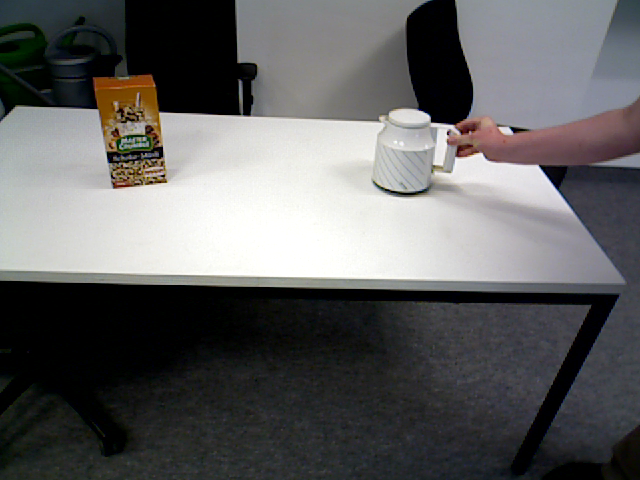
\includegraphics[width=0.22\linewidth] {evaluation/datasets/bonn_cerealbox/80}
}
\subfigure[GT Frame 40]{
   \includegraphics[width=0.22\linewidth] {evaluation/datasets/bonn_cerealbox/gt40}
}
\end{center}
\caption[Dataset Bonn Cerealbox]{An indoor scene showing a man moving a cup on table. The camera is slightly moving.}
\label{fig:eval_datasets_bonn_cerealbox}
\end{figure}
\item \textbf{Statue}: \\
\textbf{Frames}: 111, \textbf{Resolution}: $480 \times 640$, \textbf{Depths}: Yes, \textbf{Estimated Objects}: 8
\begin{figure}[H]
\begin{center}
\subfigure[Frame 30]{
   \includegraphics[width=0.22\linewidth] {evaluation/datasets/statue/30}
}
\subfigure[Frame 60]{
   \includegraphics[width=0.22\linewidth] {evaluation/datasets/statue/60}
}
\subfigure[Frame 90]{
   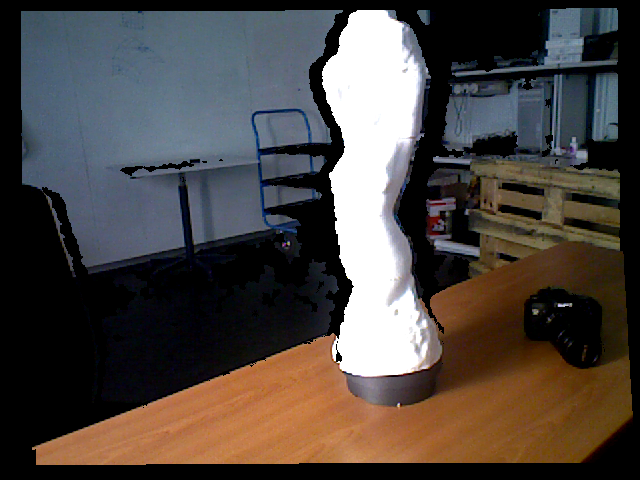
\includegraphics[width=0.22\linewidth] {evaluation/datasets/statue/90}
}
\subfigure[GT Frame 30]{
   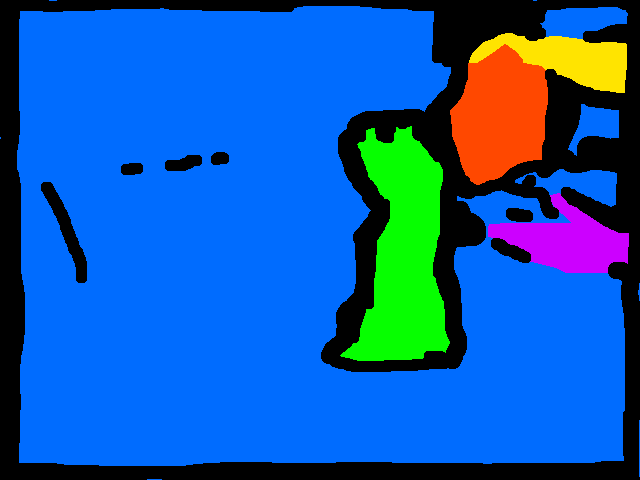
\includegraphics[width=0.22\linewidth] {evaluation/datasets/statue/gt30}
}
\end{center}
\caption[Dataset Statue]{An indoor scene a rotating statue. After a whole a man removes the upper part. We only see the man's hand. The camera is static.}
\label{fig:eval_datasets_statue}
\end{figure}
\item \textbf{Waving Arm}: \\
\textbf{Frames}: 104, \textbf{Resolution}: $480 \times 640$, \textbf{Depths}: Yes, \textbf{Estimated Objects}: 5
\begin{figure}[H]
\begin{center}
\subfigure[Frame 20]{
   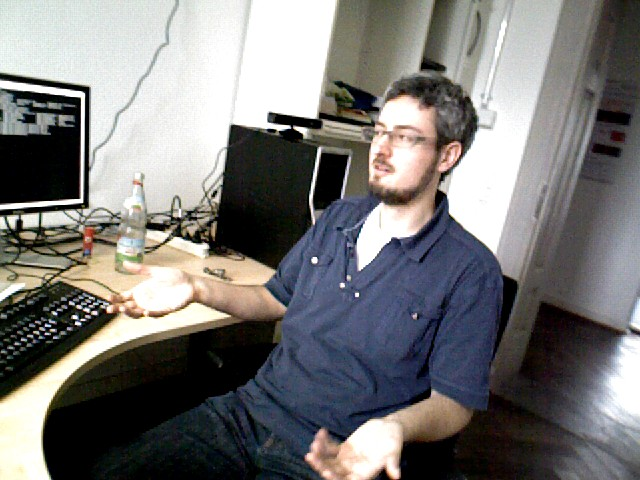
\includegraphics[width=0.22\linewidth] {evaluation/datasets/wh/20}
}
\subfigure[Frame 30]{
   \includegraphics[width=0.22\linewidth] {evaluation/datasets/wh/30}
}
\subfigure[Frame 40]{
   \includegraphics[width=0.22\linewidth] {evaluation/datasets/wh/40}
}
\subfigure[GT Frame 40]{
   \includegraphics[width=0.22\linewidth] {evaluation/datasets/wh/gt40}
}
\end{center}
\caption[Dataset Waving Hand]{An indoor scene showing a waving arm. The camera is static.}
\label{fig:eval_datasets_waving_hand}
\end{figure}
\item \textbf{Two Chairs}: \\
\textbf{Frames}: 61, \textbf{Resolution}: $512 \times 424$, \textbf{Depths}: Yes, \textbf{Estimated Objects}: 7
\begin{figure}[H]
\begin{center}
\subfigure[Frame 15]{
   \includegraphics[width=0.22\linewidth] {evaluation/datasets/two_chairs/15}
}
\subfigure[Frame 40]{
   \includegraphics[width=0.22\linewidth] {evaluation/datasets/two_chairs/40}
}
\subfigure[Frame 60]{
   \includegraphics[width=0.22\linewidth] {evaluation/datasets/two_chairs/60}
}
\subfigure[GT Frame 15]{
   \includegraphics[width=0.22\linewidth] {evaluation/datasets/two_chairs/gt15}
}
\end{center}
\caption[Dataset Two Chairs]{An indoor scene showing two spinning chairs. The camera is static.}
\label{fig:eval_datasets_two_chairs}
\end{figure}
\item \textbf{One Chair}: \\
\textbf{Frames}: 101, \textbf{Resolution}: $512 \times 424$, \textbf{Depths}: Yes, \textbf{Estimated Objects}: 7
\begin{figure}[H]
\begin{center}
\subfigure[Frame 45]{
   \includegraphics[width=0.22\linewidth] {evaluation/datasets/one_chair/45}
}
\subfigure[Frame 60]{
   \includegraphics[width=0.22\linewidth] {evaluation/datasets/one_chair/60}
}
\subfigure[Frame 75]{
   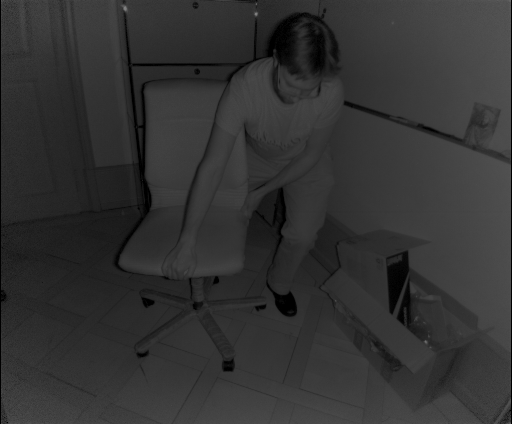
\includegraphics[width=0.22\linewidth] {evaluation/datasets/one_chair/75}
}
\subfigure[GT Frame 45]{
   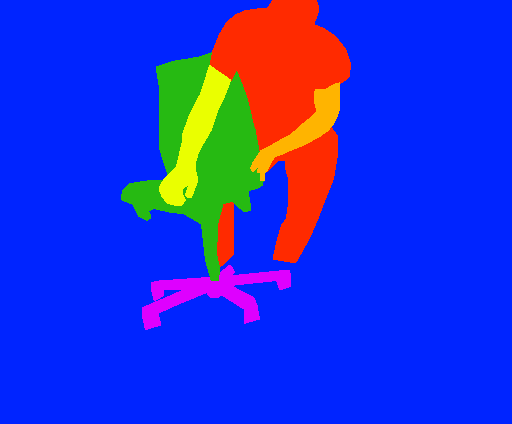
\includegraphics[width=0.22\linewidth] {evaluation/datasets/one_chair/gt45}
}
\end{center}
\caption[Dataset One Chair]{An indoor scene a man lifting a chair and spinning its lower part. The camera is static.}
\label{fig:eval_datasets_one_chair}
\end{figure}
\end{itemize}

\section{Segment Merger}
\label{sec:seg_merger}  
In this section we describe our technique to reduce oversegmentations produced by our pipeline. Our goal is to offer a mechanism that allows to evaluate the maximal potential of pipeline. However, some segmentation results are not clearly defined, such as fast movements resulting from non-rigidly moving objects. An good example of this problem case is when we attempt to segment a video showing a waving hand. That is rationale why we want to merge unclear segments. Moreover, we only allow to merger sparse segmentations, since our dense segmentation approach is basically blurring the sparse segments and thus is not yielding comparable results$\footnote{The more post-processing steps are added the more obfuscated the final segmentation quality gets.}$. This stage is invoked before running the evaluation program, implemented as a post-processing stage. \\ \\
Usually, the results generated by our pipeline exhibit an oversegmentation when comparing them against their ground truth. An example of such an oversegmentation is illustrated in Figure $\ref{fig:merger_result_b}$. Ideally, before evaluating the quality, we would like to refine our over-segmented results in a way such that the total number of unnecessary or unclear segments is reduced. Therefore we want to merge  merge segments causing an oversegmentation. We achieve this by comparing the generated segments against a manually drawn ground truth image. For any generated segment we determine their best matching ground truth segment with respect to their overlapping parts. A conceptual visualization of our merging technique is visualized in Figure $\ref{fig:merger_result}$. Please note that such a merging technique is just a hack. A more sophisticated method for merging clusters is presented in $\cite{OB14b}$.
\begin{figure}[H]
\begin{center}
\subfigure[Ground Truth Segmentation]{
   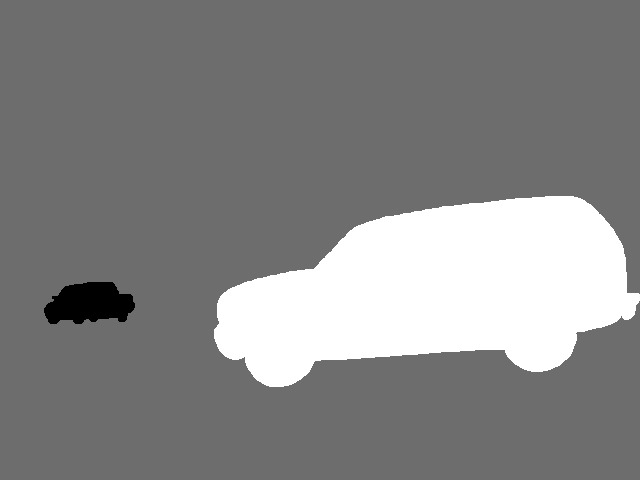
\includegraphics[width=0.47\linewidth] {implementation/merger/mask}
   \label{fig:merger_result_a}
}
\subfigure[Generated Segmentation]{
   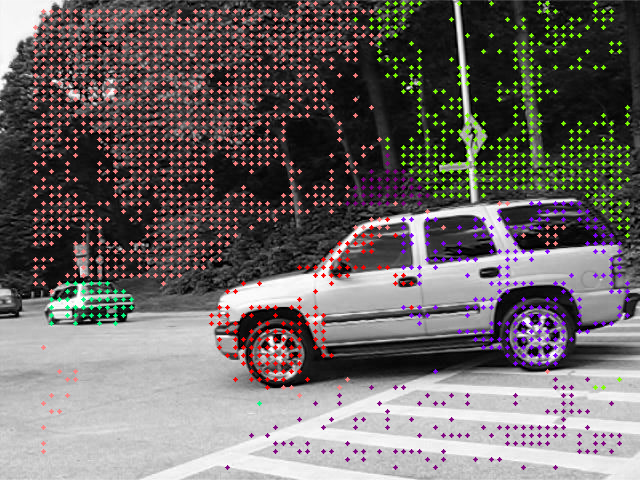
\includegraphics[width=0.47\linewidth] {implementation/merger/oversegmentation}
   \label{fig:merger_result_b}
}
~
\subfigure[Overlay Ground Truth / Segmentation]{
   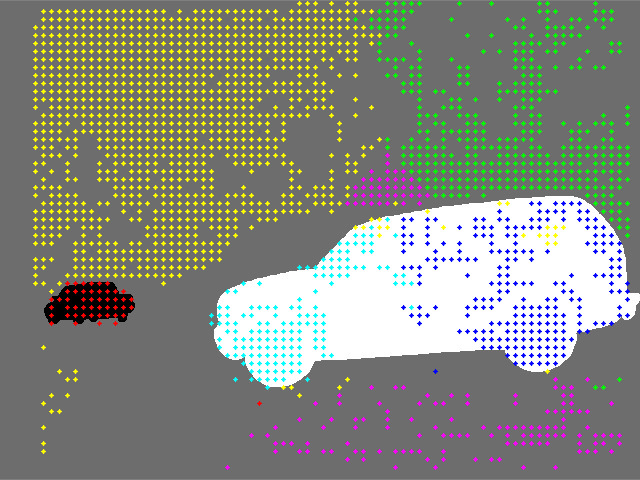
\includegraphics[width=0.47\linewidth] {implementation/merger/mask_segments_overlay}
   \label{fig:merger_result_c}
}
\subfigure[Merged Segmentation]{
   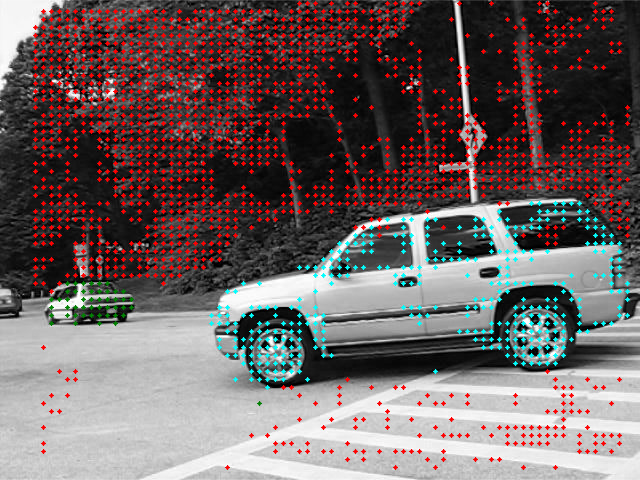
\includegraphics[width=0.47\linewidth] {implementation/merger/merged}
   \label{fig:merger_result_d}
}
\end{center}
\caption[Segmentation Merger]{Visualization of our segment merger's input and output. As an input it expects a ground truth segmentation (see Figure $\ref{fig:merger_result_a}$) and a generated oversegmentation (see Figure $\ref{fig:merger_result_b}$). As output it yields the merged segmentation as shown in Subfigure $\ref{fig:merger_result_c}$.}
\label{fig:merger_result}
\end{figure}
A segmentation $S$ is basically a set of points in which every point is assigned to a certain segment identifier. In the following let us denote $S_j$ as the subset of points in $S$ that belong to the segmentation label $j$. Similarly, let $M$ denote the set of all ground truth points with their corresponding mask labels and $M_i$ the set of all points that belong to the ground truth mask $i$. To compute the merged segments we do the following: For every segment $S_j$ in $S$ we determine its best matching ground truth segment $M_i$ as defined in Equation $\ref{eq:merging_label_formula}$. 
\begin{equation}
i = \argmaxl_{M_i \in M} \left\vert{S_j \cap M_i}\right\vert
\label{eq:merging_label_formula}
\end{equation}
The idea is to find the ground truth mask $i$ that yields the most point intersections with the currently considered segment $S_j$. Next, we update every point in $S_j$ by setting their segment label to $i$. After doing so we have computed the merged segmentation version of the initial oversegmentation. An example is shown in Figure $\ref{fig:merger_result_c}$.

\section{Methodology}
\label{sec:methodology}
In this section we give a brief description about the methodology used to perform our experiments. \\ \\
We want to quantitatively evaluate the quality of segmentations produces by running different pipeline combinations. In particular we propose to evaluate the quality of how well moving objects were segmented. We use the datasets described in Section $\ref{sec:datasets}$. Produced motion segmentations are compared against available ground truth images. While running the pipeline we rely on the defaults described in Section $\ref{sec:spectral_clustering_parameters}$.\\ \\
Before evaluating the performance of generated segmentations, we run our segment merger, which is described in Section $\ref{sec:seg_merger}$, as a post-processing step. The merged segments are quantitatively evaluated using different statistical measures. After running the merger, each GT object is assigned to at most one label. Therefore, the evaluation measures can be computed independently per object. In particular, for each segmentation result we compute their precession, recall and their f1 score by comparing them against their ground truth. The definition of these measures is listed in Equation $\ref{eq:statistical_measures}$. 
\begin{equation}
\begin{aligned}
	& \text{precision} = \frac{\text{TP}}{\text{TP} + \text{FP}} \\
	& \text{recall} = \frac{\text{TP}}{\text{TP} + \text{FN}} \\
	& F_1 \text{ Score} = 2 \left( \frac{\text{precision} \times \text{recall}}{\text{precision} +\text{recall}} \right)
\end{aligned}
\label{eq:statistical_measures}
\end{equation}
The final reported outputs is the average value of these measured over all foreground objects. \\ \\
Finally some words about how we determined the quantities $TP$, $FP$ and $FN$. We only have to iterate over all points in every cluster and compare them against an available ground image. While doing so we count their true positives (\textbf{TP}), false positives (\textbf{FP}) and their false negatives (\textbf{FN}). The exact definition of these quantities is listed in Equation $\ref{eq:statistical_counts}$. For a given label $\alpha$ these measures are defined as:
\begin{equation}
\begin{aligned}
	\textbf{TP} &:= \text{Samples correctly labeled $\alpha$} \\
	\textbf{FP} &:= \text{Samples incorrectly labeled $\alpha$} \\
	\textbf{FN} &:= \text{Samples that were labeled $\alpha$ in GT but are attributed to a wrong label.}
\end{aligned}
\label{eq:statistical_counts}
\end{equation}
A detailed explanation of these measures can be found in the background Section $\ref{sec:on_statistics_bg}$ on page $\pageref{sec:on_statistics_bg}$. \\ \\
One last note: During our evaluations we want to determine the quality of segmentations and the influence of design choices regardless of additional post-processing steps. Since our dense motion segmentation method basically performs a blurring on the sparse segmentation, and thus the quality is arbitrary influenced, we disallow using dense segmentations in our quantitative evaluation.

\section{Experiments}
\label{sec:experiments}
In this section we list the results of a series of experiments we performed running our pipeline on the presented dataset from Section $\ref{sec:datasets}$ on page $\pageref{sec:datasets}$. The results are evaluated according the previously explained measures from Section $\ref{sec:methodology}$ on page $\pageref{sec:methodology}$. \\ \\
For performing our experiments we used MacBook Pro. The hardware specifications of this machine are listed in Table $\ref{tab:used_hardware_specs}$. 
\begin{table}[H]
\centering
\begin{tabular}{|l|c|}
\hline
\multicolumn{2}{|c|}{\textbf{Hardware Specifications}} \\ \hline
\textbf{CPU} & 2.5 GHz Intel Core i7 \\ \hline
\textbf{Threads} & 8 \\ \hline
\textbf{MEMORY} & 16 GB 1600 MHz DDR3 \\ \hline
\textbf{GPU} & Intel Iris Pro 1536 MB \\ \hline
\end{tabular}
\caption{A listing of the hardware specifications of the used machine to produce the results.}
\label{tab:used_hardware_specs}
\end{table}
The first series of experiments (Sec. $\ref{sec:parameter_experiments}$) examines the influence of certain pipeline parameters. In particular we justify the choice for our default parameter assignments. Next, we study the behaviour and quality of segmentations when altering our flow estimation methods (Sec. $\ref{sec:flow_methods}$). The main experiment (Sec. $\ref{sec:overall_performance}$) is the evaluation of some strong pipeline combinations applied on all of our datasets. Finally, we perform a series of experiments to find the best pipeline combinations for each stage (Sec. $\ref{sec:pipeline_combination_cmp}$).

\subsection{Parameter Experiments}
\label{sec:parameter_experiments}
In this section we describe a series of experiments to examine our default pipeline parameters. In particular the results presented in this section act as a justification for choosing the described default values.

\subsubsection{Examine Influence of Cluster Merger}
In the following experiment we examine the influence of our cluster merger post-processing step. In particular we visually study the influence of this merging step on resulting segmentations. We generated segmentations for every LDOF pipeline combination. The results are shown in Figure $\ref{fig:eval_raw_vs_merged}$.
\begin{figure}[H]
\begin{center}
\subfigure[Raw PD SC]{
   \includegraphics[width=0.2\linewidth] {evaluation/bonn_chairs_c_10_segmentations_f_30/ldof_pd_sc}
}
\subfigure[Merged PD SC]{
   \includegraphics[width=0.2\linewidth] {evaluation/bonn_chairs_c_10/ldof_pd_sc}
}
\subfigure[Raw PD MC]{
   \includegraphics[width=0.2\linewidth] {evaluation/bonn_chairs_c_10_segmentations_f_30/ldof_pd_mc}
}
\subfigure[Merged PD MC]{
   \includegraphics[width=0.2\linewidth] {evaluation/bonn_chairs_c_10/ldof_pd_mc}
}
~
\subfigure[Raw PED SC]{
   \includegraphics[width=0.2\linewidth] {evaluation/bonn_chairs_c_10_segmentations_f_30/ldof_ped_sc}
   \label{fig:eval_bonn_chairs_raw_segmentations_frame_30_c}
}
\subfigure[Merged PED SC]{
   \includegraphics[width=0.2\linewidth] {evaluation/bonn_chairs_c_10/ldof_ped_sc}
   \label{fig:bonn_chairs_c_10_d}
}
\subfigure[Raw PED MC]{
   \includegraphics[width=0.2\linewidth] {evaluation/bonn_chairs_c_10_segmentations_f_30/ldof_ped_mc}
   \label{fig:eval_bonn_chairs_raw_segmentations_frame_30_d}
}
\subfigure[Merged PED MC]{
   \includegraphics[width=0.2\linewidth] {evaluation/bonn_chairs_c_10/ldof_ped_mc}
   \label{fig:bonn_chairs_c_10_e}
}
~
\subfigure[Raw SD KL]{
   \includegraphics[width=0.2\linewidth] {evaluation/bonn_chairs_c_10_segmentations_f_30/ldof_sd_kl}
   \label{fig:eval_bonn_chairs_raw_segmentations_frame_30_e}
}
\subfigure[Merged SD KL]{
   \includegraphics[width=0.2\linewidth] {evaluation/bonn_chairs_c_10/ldof_sd_kl}
   \label{fig:bonn_chairs_c_10_d}
}
\subfigure[Raw SED KL]{
   \includegraphics[width=0.2\linewidth] {evaluation/bonn_chairs_c_10_segmentations_f_30/ldof_sed_kl}
   \label{fig:eval_bonn_chairs_raw_segmentations_frame_30_f}
}
\subfigure[Merged SED KL]{
   \includegraphics[width=0.2\linewidth] {evaluation/bonn_chairs_c_10/ldof_sed_kl}
   \label{fig:bonn_chairs_c_10_e}
}
\end{center}
\caption[Bonn Chairs Segmentations Frame 30]{Raw-and merged segmentations produced by our pipeline when running all modes on the Bonn Chairs dataset using LDOF flow fields.}
\label{fig:eval_raw_vs_merged}
\end{figure}
From these results we can see that our pipeline tends to produce oversegmentations. Especially the steady background is clustered into meany segments. Also, the seat of the chair seems to get segmented into many parts. We also see that, after applying our merger, these parts are forming a coherent object. We conclude that our cluster merger does not significantly obfuscate the segmentation results. The corresponding statistical measurements are listed in Table $\ref{tab:eval_stat_raw_merged}$

\subsubsection{Examine Varying Cluster Count}
\label{sec:varying_cluster_exp}
In this experiment we examine the influence of a varying number of clusters on the segmentation quality. For this purpose generated segmentations on the Bonn Chairs dataset using the LDOF SED KL pipeline mode. The resulting segmentations are shown in Figure $\ref{fig:bonn_chairs_sed_varyingclusters}$ and the corresponding measurements are listed in Table $\ref{tab:bonn_chairs_ldof_sed_c_6_9_10_eval}$.
\begin{figure}[H]
\begin{center}
\subfigure[2 Clusters]{
   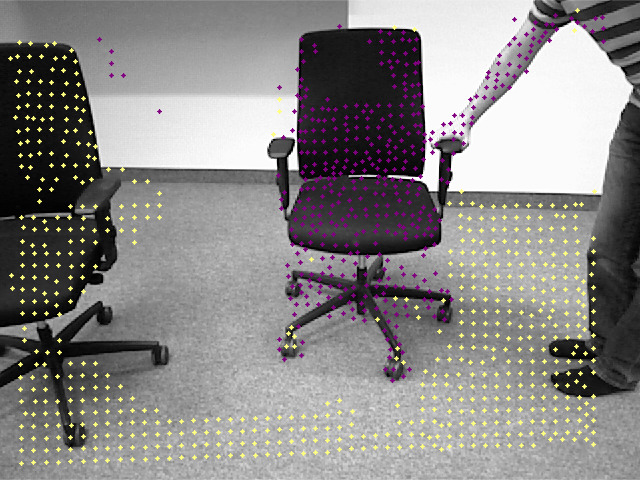
\includegraphics[width=0.31\linewidth] {evaluation/bonn_chairs_ldof_varying_c_sed/f_30_c_2}
}
\subfigure[3 Clusters]{
   \includegraphics[width=0.31\linewidth] {evaluation/bonn_chairs_ldof_varying_c_sed/f_30_c_3}
}
\subfigure[4 Clusters]{
   \includegraphics[width=0.31\linewidth] {evaluation/bonn_chairs_ldof_varying_c_sed/f_30_c_4}
}
~
\subfigure[5 Clusters]{
   \includegraphics[width=0.31\linewidth] {evaluation/bonn_chairs_ldof_varying_c_sed/f_30_c_5}
}
\subfigure[6 Clusters]{
   \includegraphics[width=0.31\linewidth] {evaluation/bonn_chairs_ldof_varying_c_sed/f_30_c_6}
}
\subfigure[7 Clusters]{
   \includegraphics[width=0.31\linewidth] {evaluation/bonn_chairs_ldof_varying_c_sed/f_30_c_7}
}
~
\subfigure[8 Clusters]{
   \includegraphics[width=0.31\linewidth] {evaluation/bonn_chairs_ldof_varying_c_sed/f_30_c_8}
}
\subfigure[9 Clusters]{
   \includegraphics[width=0.31\linewidth] {evaluation/bonn_chairs_ldof_varying_c_sed/f_30_c_9}
}
\subfigure[10 Clusters]{
   \includegraphics[width=0.31\linewidth] {evaluation/bonn_chairs_ldof_varying_c_sed/f_30_c_10}
}
\end{center}
\caption[Bonn Chairs SED Segmentations for Varying Cluster Count]{A visualization of the real segmentations when running \textit{LDOF SED KL} on the \textit{Bonn Chairs} dataset.}
\label{fig:bonn_chairs_sed_varyingclusters}
\end{figure}
We observe that using more and more clusters yields better segmentations. This trivial fact is fortified with the statistical results shown in Figure $\ref{fig:bonn_chairs_plot_avg_stat}$. To have a more solid reasoning, we additionally evaluated LDOF PD SC and LDOF PED MC for a varying number of clusters and generated their corresponding performance graphs.
\begin{figure}[H]
\begin{center}
\subfigure[Recall / Precision Plot]{
   \includegraphics[width=0.47\linewidth] {evaluation/bonn_chairs/avg/avg_rec_prec}
}
\subfigure[Cluster Count / F1 Score Plot]{
   \includegraphics[width=0.47\linewidth] {evaluation/bonn_chairs/avg/avg_clusters_f1}
}
\end{center}
\caption[Bonn Chairs Varying Clusters]{Visualizing plots of the average performance of the combinations LDOF PD SC (Tab. $\ref{tab:bonn_chairs_ldof_sed_c_6_9_10_eval_pd_sc}$), LDOF PED MC (Tab. $\ref{tab:bonn_chairs_ldof_sed_c_6_9_10_eval_ped_mc}$) and LDOF SED KL (Tab. $\ref{tab:bonn_chairs_ldof_sed_c_6_9_10_eval}$) for a varying number of clusters. The left plots shows the recall/precision plot and the figure on the right shows the F1 score alongside the number of clusters.}
\label{fig:bonn_chairs_plot_avg_stat}
\end{figure}

\subsubsection{Examine Convergence of MC}
In this experiment we have a closer look at the convergence rate of the Minimum Cut (MC) segmentation method (Sec. $\ref{sec:min_cut_seg}$). For this purpose we run the mode LDOF PED MC on the Two Chairs dataset. Moreover, we set the cluster count to 20. On one hand, using that many clusters will result in producing oversegmentations but on the other hand this also ensures a good convergence rate plot (due to our segment merger). The graph in Figure $\ref{fig:convergence_rate_mc}$ visualizes the convergence rate of the MinCut (MC) segmentation technique. The corresponding measurements are listed in Table $\ref{tab:two_chairs_ped_mc_iterations}$
\begin{figure}[H]
\begin{center}
\includegraphics[width=0.47\linewidth] {evaluation/two_chairs/performance_iter/iter_f1}
\end{center}
\caption[Convergence Rate MinCut Segmentation]{Visualizing the convergence rate of Minimum Cut when running LDOF PED MC. We observe, that the more iterations are run, the higher the F1-Score gets. However}
\label{fig:convergence_rate_mc}
\end{figure}
We observe that the more iterations we run, the higher the F1-Score gets. However, we also observe, that the F1 Score is converging already after 4 iterations. This matches with our assumption that no more than 20 iterations have to be run when using the MC segmentation method.

\begin{figure}[H]
\begin{center}
\subfigure[1 Iteration]{
   \includegraphics[width=0.22\linewidth] {evaluation/two_chairs/iters/iter_1}
}
\subfigure[2 Iterations]{
   \includegraphics[width=0.22\linewidth] {evaluation/two_chairs/iters/iter_2}
}
\subfigure[3 Iterations]{
   \includegraphics[width=0.22\linewidth] {evaluation/two_chairs/iters/iter_3}
}
\subfigure[5 Iterations]{
   \includegraphics[width=0.22\linewidth] {evaluation/two_chairs/iters/iter_5}
}
\end{center}
\caption[Convergence Segmentations Two Chairs]{Visualizing the convergence of the MC segmentation method.}
\label{fig:two:chairs_segmentations_ped_mc_iters_exp}
\end{figure}

\subsubsection{Examine $\lambda$ Default}
In this experiment we examine the influence of the parameter $\lambda$, which is used to scale P-affinities. In particular, we try legitimize our standard $\lambda$ choices. In the following we use the Bonn datasets and evaluate the quality of LDOF PD SC and LDOF PED SC for different $\lambda$ values. The averaged statistics are listed in Table $\ref{tab:varying_lambda_experiment}$.
\begin{table}[H]
\centering
\setlength\tabcolsep{4pt}
\begin{minipage}{0.48\textwidth}
\centering
\begin{tabular}{|c|c|c|c|}
\hline
\multicolumn{4}{|c|}{Varying $\lambda$ on PD} \\ \hline
$\lambda$ & \textbf{Precision} & \textbf{Recall} & \textbf{F1 Score} \\ \hline
5 & 11.68 & 10.73\% & 11.18\%  \\ \hline
1 & 15.68 & 11.51\% & 13.28\%  \\ \hline
0.1 & 34.05 & 30.08\% & 31.94\%  \\ \hline
\textbf{0.01} & \textbf{46.37} & \textbf{52.94}\% & \textbf{49.44}\%  \\ \hline
0.001 & 43.00 & 45.67\% & 44.29\%  \\ \hline
0.0001 & 25.11 & 25.78\% & 25.44\%  \\ \hline
\end{tabular}
\end{minipage}%
\hfill
\begin{minipage}{0.48\textwidth}
\centering
\begin{tabular}{|c|c|c|c|}
\hline
\multicolumn{4}{|c|}{Varying $\lambda$ on PED}                        \\ \hline
$\lambda$ & \textbf{Precision} & \textbf{Recall} & \textbf{F1 Score} \\ \hline
100 & 36.60\% & 35.11\% & 35.84\%  \\ \hline
\textbf{50} & \textbf{52.44}\% & \textbf{59.28}\% & \textbf{55.65}\%  \\ \hline
10 & 45.33\% & 52.22\% & 48.53\%  \\ \hline
5 & 53.50\% & 51.02\% & 52.23\%  \\ \hline
1 & 47.58\% & 43.50\% & 45.45\%  \\ \hline
0.1 & 44.75\% & 41.00\% & 42.79\%  \\ \hline
\end{tabular}
\end{minipage}
\caption[Experiment Varying $\lambda$]{The averaged statistics of a varying $\lambda$ on P-affinities applied on the Bonn datasets. On the left table, the results when using PED affinities, on the right, when using PD affinities. The best determined choices for $\lambda$ are marked in bold face.}
\label{tab:varying_lambda_experiment}
\end{table}
We observe that $\lambda$ equals $0.01$ works best for PD affinities and when $\lambda = 50$ when using PED affinities \\ \\
In the following we visualize the influence of $\lambda$ on the segmentation quality. For this purpose we produced PD SC segmentations on the Cars dataset for different $\lambda$ values. The resulting segmentations are shown in Figure $\ref{fig:cars_dataset_lambdas}$.
\begin{figure}[H]
\begin{center}
\subfigure[$\lambda$ = 5]{
   \includegraphics[width=0.31\linewidth] {evaluation/cars/lambdas/5}
   \label{fig:cars_dataset_lambdas_a}
}
\subfigure[$\lambda$ = 0.01]{
   \includegraphics[width=0.31\linewidth] {evaluation/cars/lambdas/0_01}
   \label{fig:cars_dataset_lambdas_b}
}
\subfigure[$\lambda$ = 0.0001]{
   \includegraphics[width=0.31\linewidth] {evaluation/cars/lambdas/0_0001}
   \label{fig:cars_dataset_lambdas_c}
}
~
\subfigure[Undersegmented]{
   \includegraphics[width=0.31\linewidth] {evaluation/cars/lambdas/seg_5}
   \label{fig:cars_dataset_lambdas_a}
}
\subfigure[Ideal]{
   \includegraphics[width=0.31\linewidth] {evaluation/cars/lambdas/seg_0_01}
   \label{fig:cars_dataset_lambdas_b}
}
\subfigure[Oversegmented]{
   \includegraphics[width=0.31\linewidth] {evaluation/cars/lambdas/seg_0_0001}
   \label{fig:cars_dataset_lambdas_c}
}
\end{center}
\caption[Influence varying $\lambda$]{Illustration of the influence of the parameter $\lambda$ used to scale PD-affinities. The first row shows the affinities between a certain trajectory on the car on the back (marked by a red circle) and its neighbors. The second row shows the corresponding segmentations.}
\label{fig:cars_dataset_lambdas}
\end{figure}
As we can see, the optimal value $\lambda = 0.01$ produced the best segmentation. Moreover, a too large value leads to an oversegmentation, but when using a too small value we obtain an undersegmentation. These results allow us to conclude that our $\lambda$ defaults are reliable enough to use them during our experiments.

\subsubsection{Examine Eigenvector-/Cluster-Count Defaults}
In Section $\ref{sec:spectral_clustering_parameters}$ we mentioned what default values we use for the number of clusters and eigenvectors, when either running the SC or the MD segmentation method. We stated, that we use twice the estimated count of the moving objects present in the video as the cluster count and twice the cluster count as the number of eigenvalues. In order to legitimize the usage of those defaults, we created a series of segmentations for a varying number of clusters and eigenvectors. \\ \\
In this experiment we evaluate the Cars dataset, since it has a static camera and a known number of large moving objects. In particular, there are two moving cars, each forming a moving objects and the background. Therefore we use the estimate \textit{3 segments}. Moreover, we use the optimal $\lambda$ value for PD affinities. Finally, we run the SC segmentation method on every cluster-/eigenvector-count combination between 3 to 6 clusters and 3 to 12 eigenvectors. To ease the readability of the results, we produced two graphs as shown in Figure $\ref{fig:cc_ev_combinations}$. The graph on the left plots the f1 score against a fixed number of clusters and a varying number of eigenvectors. In contrast, the graph on the right side fixes the number of used eigenvectors but keeps the cluster count as a free variable.
\begin{figure}[H]
\begin{center}
\subfigure[Fixed Clusters and Varying Eigenvectors]{
   \includegraphics[width=0.444\linewidth] {evaluation/exploring_params/free_ev}
}
\subfigure[Fixed Eigenvectors and Varying CC]{
   \includegraphics[width=0.505\linewidth] {evaluation/exploring_params/free_cc}
}
\end{center}
\caption[Varying number of Clusters / Eigenvectors]{Two graphs that show the f1 score for a varying number of clusters and eigenvectors on the cars dataset. The graph on the left shows plots for fixed cluster numbers and the graph on the right plots the f1 score for a fixed eigenvalue count and varying cluster counts.}
\label{fig:cc_ev_combinations}
\end{figure}
At first glance, the resulting graphs seem to have a very complicated behaviour. We observe oscillations in the f1 scores, when increasing the number of clusters. This behaviour seems to be counterintuitive. Hence, the optimal cluster/eigenvalue count choice seems to be more complex than our simple heuristic. However, when considering the fixed clusters graph, we observe that our assumption to use \textit{6 clusters} ranks amongst the best variants. Moreover, when considering the plots for fixed eigenvectors, then we see that using 6 clusters together with 12 eigenvectors also yields top results. \\ \\
However, we also notice, that this assumption may not be the best variant, since other cluster-eigenvector combinations also produce top results, according to the f1 score. Despite this last observation we can conclude, that our defaults for the cluster- and and eigenvector count allow to produce good results. Therefore we will use this cluster and eigenvector heuristic during this evaluation. \\ \\
Additional \enquote{varying the cluster-eigenvalue count} experiments and their measurements can be found in the appendix in Section $\ref{sec:additional_cc_ev_exp}$.

\subsection{On Exploring Flow Methods}
\label{sec:flow_methods}
Evaluating every pipeline combination on every dataset would exceed our capabilities, since there are simply too many cross-combinations. Therefore, we would like to detect and filter some weak combinations in advance. By having a closer look at the performance on the flow methods, we will be able to drop two methods. \\ \\
In this section we examine the quality of the utilized flow methods. In particular we show that the flow methods HS and LRGBD do not produce good estimates and thus can be dropped from further considerations during our series of experiments. This will reduce the total number of pipeline combinations by a factor of two. \\ \\
In the first sub-experiment we compare the segmentations produced on LDOF-and HS flow fields. In the second experiment we examine the quality of segmentations produced by LRGBD flow fields.

\subsubsection{LDOF vs. HS Flow Fields}
Both flow estimation methods, LDOF and HS, are not making use of depth fields. Therefore, we would like to determine whether one of these two methods is significantly better. \\ \\
In the following experiment we compute P-affinities using LDOF and HS flow fields on the Bonn datasets. In order to examine the quality of the flow fields, we evaluate SC segmentations using these affinities. The average statistics are listed in Table $\ref{tab:hs_vs_ldof}$.
\begin{table}[H]
\centering
\begin{tabular}{|c|c|c|c|}
\hline
\multicolumn{4}{|c|}{LDOF vs. HS on Bonn Datasets}                        \\ \hline
Method & \textbf{Precision} & \textbf{Recall} & \textbf{F1 Score} \\ \hline
LDOF PD SC & 42.98\%   & 55.06\%     & 48.28\%  \\ \hline
HS PD SC MC & 40.19\%   & 52.33\%     & 45.47\%  \\ \hline
LDOF PED SC & 69.34\%   & 54.13\%     & 60.80\%  \\ \hline
HS PED SC MC & 55.61\%   & 53.15\%     & 54.35\%  \\ \hline             
\end{tabular}
\caption[LDOF vs. HS Flow Fields]{Comparison of Bonn dataset segmentations produced by running PD SC and PED SC on LDOF- and HS flow fields. Methods using LDOF flow fields seem to be produce better segmentations than those which are using HS flow fields.}
\label{tab:hs_vs_ldof}
\end{table}
Apparently, pipeline combinations that use LDOF flow fields are producing qualitatively better segmentations than those which use HS flow fields. Therefore, we decide to drop HS flow fields and only use LDOF flow fields instead.

\subsubsection{On LRGBD Flow Fields}
In the following we want to examine the quality of segmentations that use LRGBD, LDOF and SRSF flow fields on the Statue dataset. For this purpose we vary the used flow method and fix the pipeline mode to PED MC. Hence, we run the following three combinations: LDOF PED MC, SRSF PED MC, LGBDR PED MC. \\ \\
The achieved performances are listed in Table $\ref{tab:statue_performance}$ and visual segmentations are depicted in Figure $\ref{fig:alley_segmentations}$.
\begin{table}[H]
\centering
\begin{tabular}{|c|c|c|c|}
\hline
\multicolumn{4}{|c|}{Performance Statue dataset}                        \\ \hline
Method & \textbf{Precision} & \textbf{Recall} & \textbf{F1 Score} \\ \hline
LDOF PED MC & 69.93\%   & 38.23\%     & 49.44\%  \\ \hline
SRSF PED MC & 72.47\%   & 70.68\%     & 71.56\%  \\ \hline
LRGBD PED MC & 61.46\%   & 8.37\%     & 14.73\%  \\ \hline              
\end{tabular}
\caption[Performance Statue]{Comparing the segmentation quality produced by LDOF, SRSF and LRGBD flow fields.}
\label{tab:statue_performance}
\end{table}
We observe that segmentations that use SRSF flow fields score good, and segmentations using LDOF fields score intermediate quality results. However, pipeline combinations based on LRGBD flow fields produce visually, as well as statistically very poor segmentations. Apparently, this flow method is a bad choice for the task of motion segmentation. Therefore, we drop it from our pipeline. 
\begin{figure}[H]
\begin{center}
\subfigure[LDOF PED MC]{
   \includegraphics[width=0.31\linewidth] {evaluation/statue/segmentations/f30/ldof_ped_mc}
   \label{fix:alley_segmentations_a}
}
\subfigure[SRSF PED MC]{
   \includegraphics[width=0.31\linewidth] {evaluation/statue/segmentations/f30/srsf_ped_mc}
   \label{fix:alley_segmentations_b}
}
\subfigure[LGBDR PED MC]{
   \includegraphics[width=0.31\linewidth] {evaluation/statue/segmentations/f30/lrgbd_ped_mc}
   \label{fix:alley_segmentations_c}
}
~
\subfigure[LDOF PED MC]{
   \includegraphics[width=0.31\linewidth] {evaluation/statue/segmentations/f60/ldof_ped_mc}
   \label{fix:alley_segmentations_d}
}
\subfigure[SRSF PED MC]{
   \includegraphics[width=0.31\linewidth] {evaluation/statue/segmentations/f60/srsf_ped_mc}
   \label{fix:alley_segmentations_e}
}
\subfigure[LGBDR PED MC]{
   \includegraphics[width=0.31\linewidth] {evaluation/statue/segmentations/f60/lrgbd_ped_mc}
   \label{fix:alley_segmentations_f}
}
\end{center}
\caption[Bonn Cerealbox Segmentations]{Visualization of the segmentation that belong to the results listed in Table $\ref{tab:statue_performance}$.}
\label{fig:alley_segmentations}
\end{figure}
Although the LRGBD flow fields are supposed to be competitive against SRSF flow fields, using them in segmentation tasks yields qualitatively poor segmentations. This is due the fact, that LRGBD flow fields are estimated by segmenting the flow fields with respect to their depth layers instead according to their motion. \\ \\
In order to verify that \enquote{LRGBD flow fields are indeed not suitable for our motion segmentation pipeline}, we performed a second experiment: This time we evaluated the Bonn Watercan segmentations. We used all existing flow methods and produced segmentations using PED-affinities. The results are listed in Table $\ref{tab:bonn_wc_flwo_methods}$.
\begin{table}[H]
\centering
\begin{tabular}{|l|r|l|l|}
\hline
\multicolumn{4}{|c|}{Flow Comparison on Bonn Watercan Dataset} \\ \hline
& \textbf{Precision} & \textbf{Recall} & \textbf{F1 Score} \\ \hline            
HS PED SC  & 71.59\%   & 71.96\%     & 71.77\%  \\ \hline
HS PED MC  & 71.84\%   & 72.59\%     & 72.21\%  \\ \hline                        
LDOF PED SC  & 94.30\%   & 58.20\%     & 71.98\%  \\ \hline
LDOF PED MC  & 67.50\%   & 81.06\%     & 73.66\%  \\ \hline
SRSF PED SC & 90.00 \%   & 96.25\%     & 93.02\%  \\ \hline
SRSF PED MC & 94.23 \%   & 95.04\%     & 94.63\%  \\ \hline
LRGBD PED SC & 30.00\%   & 16.68\%     & 21.43\%  \\ \hline
LRGBD PED MC & 31.23\%   & 16.32\%     & 21.44\%  \\ \hline
\end{tabular}
\caption[Flow Method Comparission on Bonn Watercan]{Comparing the quality of our flow methods on the Bonn Watercan dataset.}
\label{tab:bonn_wc_flwo_methods}
\end{table}
Again, we observe, that LRGBD flow fields produce poor segmentations. So, what is going on there? To get a better understanding of the underlying problem, we have a look at the actual segmentations produced by the combination LRGBD PED MC. The corresponding segmentation of frame 30 is visualized in Figure $\ref{fig:issues_lrgbd_flow_methods}$. 
\begin{figure}[H]
\begin{center}
\subfigure[Extracted Layers Frame 30]{
   \includegraphics[width=0.31\linewidth] {evaluation/lrgbd_issues/layers_30}
   \label{fig:issues_lrgbd_flows_a}
}
\subfigure[Forward Flow Frame 30]{
   \includegraphics[width=0.31\linewidth] {evaluation/lrgbd_issues/fw_flow_30}
   \label{fig:issues_lrgbd_flows_b}
}
\subfigure[Segmentation PED MC Frame 30]{
   \includegraphics[width=0.31\linewidth] {evaluation/lrgbd_issues/seg_30}
   \label{fig:issues_lrgbd_flows_c}
}
\end{center}
\caption[Issue with LRGBD Flow Fields]{Comparing the a LRGBD based segmentation against its flow field.}
\label{fig:issues_lrgbd_flow_methods}
\end{figure}
We notice that the LRGBD flow fields are locally homogenous within the layer they belongs to. Moreover, LRGBD segmentations separate the objects according to their depth layers rather than by their motion.

\subsection{Overall Performance}
\label{sec:overall_performance}
So far, we justified our default parameter choices and we were able to drop two poorly behaving flow methods (HS and LRGBD). In this experiment, we want to evaluate the segmentation quality of all LDOF and SRSF pipeline combinations applied on five datasets (Cerealbox, Chairs, Watercan, Waving-Arm and Statue). Unfortunately, we cannot use every dataset in this experiment because not every pipeline method can be run on every available dataset. For instance, SRSF flow fields can only be generated for images with a resolution of $640 \times 480$ pixels. Furthermore, we only use datasets that have measured depth fields.\\ \\
In particular we are interested in comparing the modes LDOF PD SC and SRSF PED MC, since the first combination resembles to the implementation described in $\cite{OB14b}$$\footnote{Both implementations use LDOF flow fields, a similar affinity measure and a similar spectral clustering technique.}$ and the second is supposed to be our best P-affinity variant. Moreover, we used $\cite{KB15b}$' GraphCut$\footnote{This method does not use depth data.}$ implementation and let it compete against our pipeline. The averaged f1 scores of this experiment is visualized in Figure $\ref{fig:overall_performance_bar_chart}$. The corresponding measurements are listed in Table $\ref{tab:overall_performance}$.
\begin{figure}[H]
\begin{center}
\includegraphics[width=0.7\linewidth] {evaluation/overall/all}
\end{center}
\caption[Overall Performance Bar Chart]{Evaluation of LDOF and SRSF flow fields using all pipeline combinations on all compatible datasets.}
\label{fig:overall_performance_bar_chart}
\end{figure}
We observe the following facts: 
\begin{itemize}
	\item Combinations that use SRSF flow fields achieve better results than those that use LDOF flow fields.
	\item Methods that make use of depth cues are generally performing better than two dimensional approaches.
	\item Lastly, using the Minimum Cut (MC) segmentation technique produces better results than spectral clustering (SC)
\end{itemize}
Overall, The Kernighan-Lin (KL) heuristic yields the best segmentations among all segmentation methods. Lastly, Brox's GraphCut does not produce very good segmentation results. However, to be fair, we used its standard parameters but used optimal parameters in our pipeline (determined for the used datasets). Additionally, we evaluated all LDOF P-affinity pipeline combinations on every dataset. The results are listed in Table $\ref{tab:overall_performance_ldof}$.
\begin{table}[H]
\centering
\begin{tabular}{|c|c|c|c|}
\hline
\multicolumn{4}{|c|}{LDOF on every datasets}                        \\ \hline
Method & \textbf{Precision} & \textbf{Recall} & \textbf{F1 Score} \\ \hline
LDOF PD SC & 63.52 \%   & 41.87\%     & 50.47\%  \\ \hline
LDOF PD MC & 58.69\%   & 57.86\%     & 58.27\%  \\ \hline
LDOF PED SC & 66.94\%   & 57.91\%     & 62.10\%  \\ \hline
LDOF PED MC & 64.11\%   & 67.27\%     & 65.65\%  \\ \hline                 
\end{tabular}
\caption[Overall Performance LDOF P-Affinities]{Evaluation of all LDOF-P-affinity pipeline combinations on every dataset. }
\label{tab:overall_performance_ldof}
\end{table}
From these measurements we observe again, that incorporating depths (via running PED) into the pipeline yields significant better results than without doing so. Moreover, MC achieves higher f1 scores than SC. 

\subsection{Pipeline Combination Comparisons}
\label{sec:pipeline_combination_cmp}
Our pipeline allows to alter between many different flow estimation-, affinity matrix computation- and segmentation methods. In this section we want to determine an optimal pipeline combination by comparing the methods of each stage and choosing the best one.

\subsubsection{LDOF vs. SRSF}
In this section we want to illustrate the dominance of SRSF flow fields. For this purpose we evaluated the segmentations of the Bonn datasets. In this experiment we strictly use the MC segmentation method and generated segmentations for all P-affinity measures. The results are listed in Table $\ref{tab:bonn_datasets_ldof_vs_srsf}$.
\begin{table}[H]
\centering
\begin{tabular}{|l|c|c|c|}
\hline
\multicolumn{4}{|c|}{Comparison flow fields Bonn dataset using MC}                        \\ \hline
\textbf{Method} & \textbf{Precision} & \textbf{Recall} & \textbf{F1 Score}  \\ \hline
LDOF PD & 35.76\% & 46.90\% & 40.58\% \\ \hline
SRSF PD & 48.32\% & 48.99\% & 48.65\% \\ \hline
LDOF PED & 44.22\% & 50.92\% & 47.34\% \\ \hline
SRSF PED & 81.88\% & 59.32\% & 68.80\% \\ \hline
\end{tabular}
\caption[LDOF vs. SRSF: Bonn Datasets]{Comparing segmentations on LDOF and SRSF flow fields using MC}
\label{tab:bonn_datasets_ldof_vs_srsf}
\end{table}
We observe that segmentations based on SRSF flow fields always obtain higher f1 scores. Therefore, using SRSF flow fields seems to be beneficial.

\subsubsection{2D vs. 3D}
In this section we want to illustrate the dominance of affinities that incorporate depth measurements. For this purpose we evaluated the segmentations of the Bonn Chairs dataset. In this experiment we strictly use LDOF flow fields and generated segmentations for every possible pipeline mode. The results are listed in Table $\ref{tab:bonn_datasets_2d_vs_3d}$.
\begin{table}[H]
\centering
\begin{tabular}{|l|c|c|c|}
\hline
\multicolumn{4}{|c|}{Comparison Bonn Chairs on LDOF}                        \\ \hline
\textbf{Method} & \textbf{Precision} & \textbf{Recall} & \textbf{F1 Score}  \\ \hline
LDOF PD SC & 47.48\% & 54.88\% & 50.91\% \\ \hline
LDOF PED SC & 56.86\% & 55.35\% & 55.35\% \\ \hline
LDOF PD MC & 46.46\% & 63.10\% & 53.51\% \\ \hline
LDOF PED MC & 56.68\% & 64.56\% & 60.36\% \\ \hline              
LDOF SD KL & 51.34\% & 63.44\% & 56.75\% \\ \hline
LDOF SED KL & 68.42\% & 69.63\% & 69.01\% \\ \hline
\end{tabular}
\caption[2D vs. 3D: Bonn Datasets]{Comparing affinities computed by 3D trajectories against 2D trajectories.}
\label{tab:bonn_datasets_2d_vs_3d}
\end{table}
We observe that, regardless of the choice of segmentation method, affinities produced by using depths achieve higher f1 scores than does without. Therefore, using depths seems to be beneficial.

\subsubsection{SC vs. MC}
In this experiment we compare our two P-affinity segmentation methods, SC and MC. For this purpose we strictly used LDOF flow fields and evaluated the generated segmentations of the following combinations: PD SC, PD MC, PED SC and PED MC. The corresponding results are listed in Table $\ref{tab:one_chair_sc_vs_mc}$
\begin{table}[H]
\centering
\begin{tabular}{|l|c|c|c|}
\hline
\multicolumn{4}{|c|}{Comparison one Chair dataset on LDOF}                        \\ \hline
\textbf{Method} & \textbf{Precision} & \textbf{Recall} & \textbf{F1 Score}  \\ \hline
LDOF PD SC & 54.23\% & 47.82\% & 50.82\% \\ \hline
LDOF PD MC & 55.64\% & 49.50\% & 52.39\% \\ \hline
LDOF PED SC & 56.14\% & 53.75\% & 54.92\% \\ \hline
LDOF PED MC & 62.23\% & 58.07\% & 60.08\% \\ \hline              
\end{tabular}
\caption[SC vs. MC]{Comparing the segmentation methods SC and MC} 
\label{tab:one_chair_sc_vs_mc}
\end{table}
We observe, that segmentations produced by MC always obtain higher f1 scores than SC methods. It seems beneficial to use the MC segmentation method when using P-affinities.

\section{Runtime Measurements}
\label{sec:runtime_measurements}
In this section we present a series of runtime measurements on our pipeline when using the machine described in Table $\ref{tab:used_hardware_specs}$. Note that by no means, these measurements can be considered as statistical evident. The sole purpose of this section is to offer the reader some further insights about the pipeline and its usability in terms of \textit{how handy is this whole pipeline to use w.r.t. its runtime}. \\ \\
We start with measuring the runtimes of the utilized flow methods. For each method we run three dataset$\footnote{The dataset frames used to perform these measurement all exhibit a resolution 640 x 480 pixels.}$ and measured their total required time to process their input. Each measurement was divided by the total number of used frames. The final resulting timings are the average of these measurements. Table $\ref{flow_method_runtimes}$ lists the average time in seconds that our flow methods require to process$\footnote{Here, the term process refers to generating the forward-and backward flow field of a frame.}$ one dataset frame. 
\begin{table}[H]
\centering
\begin{tabular}{|l|c|}
\hline
\textbf{Flow Method} & \textbf{Time per Frame} \\ \hline
HS & 18s \\ \hline
LDOF & 24s \\ \hline
SRSF & 72s \\ \hline
LRGBD & 674s \\ \hline
\end{tabular}
\caption[Flow Method Runtimes]{Listing of the average time of our flow methods required to process one dataset frame}
\label{flow_method_runtimes}
\end{table}
Next, let us discuss the timings of the affinity matrix generation. Figure $\ref{fig:runtime_tra_track_affinity_gen}$ shows the timings in seconds of 261 measurements (blue dots) to accomplish the task of tracking a varying count of trajectories and generating their corresponding affinity matrix. Moreover, we fit a quadratic polynomial (red curve) on our measurements, since the runtime complexity of this pipeline stage is supposed to be in $\mathcal{O}(n^2)$ and $n$ denotes the trajectory count.
\begin{figure}[H]
\begin{center}
\includegraphics[width=0.8\linewidth] {evaluation/runtimes/affinity}
\end{center}
\caption[Runtime Trajectory Tracking and Generating Affinity Matrix]{Plotting the runtime (in seconds) of trajectory tracking and affinity matrix generation stage against the utilized trajectory count. The measurements are visualized as blue dots. A reconstructed quadratic curve is shown in red. The runtime of the evaluated stage is supposed to exhibit a quadratic complexity.}
\label{fig:runtime_tra_track_affinity_gen}
\end{figure}
Unfortunately, we have not performed detailed measurements for the $\textit{P-affinity}$ segmentation methods. In our pipeline, we implemented the Spectral Clustering (SC) and Minimum Cut (MC) segmentation methods in Matlab. Generally, loading an affinity matrix, that represents the similarity of 1000 affinities, takes 5 seconds, 3000 approximately 20 seconds and 6000 about 120 seconds. For solving the eigenvalue decomposition in our Matlab implementations, we rely on the fast numerical approximation of $\textit{eigs}$. The final k-means run in SC takes about 30 seconds when applied on 6000 trajectories and running 200 repetitions. \\ \\
The most outer loop in the MC implementation runs a k-means step and a graph-cut step. The k-means step takes about the same time as it does in SC. Again, when using about 6000 trajectories and the default neighborhood assignment as discussed in Section $\ref{sec:spectral_clustering_parameters}$, then calling graph-cut in this loop takes about 3 minutes. \\ \\
We measured the timings of several Kerninghan-Lin runs. For a fixed number of neighbors, the overall runtime of the KL algorithm depends on the number of trajectories and the number of iterations. The number of iterations is determined by the number of clusters CC we want to solve for and is defined as
\begin{equation}
	\text{Iters} = \sum_{k=1}^{\text{CC}-1} k
\end{equation}
which corresponds to the number of all possible distinct pair formations. The resulting measurement graph is shown in Figure $\ref{fig:runtime_kl_graph_part}$.
\begin{figure}[H]
\begin{center}
\includegraphics[width=0.8\linewidth] {evaluation/runtimes/kl}
\end{center}
\caption[Runtime KL Graph Partitioning]{Visualizing of the runtimes in seconds of KL vs. the product between the number of the used trajectories times the number of iterations. As we can see, KL is takes a lot of time when trying to solve for many clusters and many trajectories the same time.}
\label{fig:runtime_kl_graph_part}
\end{figure}
As we can see, running KL is very time consuming. For instance, when we use a large number of clusters, say 10 clusters, and using approximately 5000 trajectories, then this algorithm takes about 7000 seconds to finish.

\section{Discussion}
\label{sec:discussion}
In the previous section we performed a series of experiments on different datasets to examine the influence of various pipeline components and their corresponding parameters. In this section we list the main findings of those experiments and relate them to our initial thesis goals. \\ \\
We visually and statistically demonstrated that our pipeline is able to produce good segmentation results on complex scenes. In particular, our best pipeline combination could handle scenes consisting of moving cameras and rotating moving objects. Therefore, we achieved our initial goal of building a motion segmentation pipeline on RGB-D videos using optical flow fields. \\ \\
Our motion segmentation pipeline is an over-parameterized multi-stage implementation. Usually, finding the correct parameter values is not obvious. We therefore suggested reliable heuristics to specify some of the parameters. In our experiments we were able to justify our default parameter choices. \\ \\
We further were able to determine the best pipeline combinations. We experimentally demonstrated that SRSF flow fields outperform every other flow method supported by our pipeline. Moreover, we successfully could show that using depth information drastically increases the quality of resulting motion segmentations. Among our segmentation methods, KL produces the best results. This method, however, uses S-affinities. In contrast, when using P-affinities, MC seems the be the best choice. When comparing KL against MC we can conclude, that KL produces better results but at the same time requires an enormous amount of computation time. In contrast, MC runs in a decent time and at the same time produces good and convincing results. By combining all these findings, we nominate the two following winner combinations: SRSF PED MC and SRSF SED KL. \\ \\
Additionally, we let our pipeline compete against Brox' GraphCut $\cite{KB15b}$, which corresponds to the pipeline combination $\textit{LDOF SD KL}$. Interestingly, every pipeline combination obtains better results even when not using depth data. However, to be fair, we have to mention that we did not specify any specific GraphCut parameters and hence his implementation was using its standard setup. In contrast, we used optimal parameters for our implementations during the experiments. \\ \\
Additional experiments and corresponding results can be found in the appendix Chapter $\ref{chap:additional_exp}$.
